

\begin{frame}{Current Status}
  \begin{center}
    \Large PETSc on GPUs and MIC: \\[1em] Current Status
  \end{center}
\end{frame}

\begin{frame}[fragile]
\frametitle{Available Options}

 \begin{minipage}{0.75\textwidth}
  \begin{block}{Native on Xeon Phi}
  \begin{itemize}
   \item Cross-compile for Xeon Phi
  \end{itemize}
  \end{block}

  \begin{block}{CUDA}
  \begin{itemize}
   \item CUDA-support through CUSP
   \item \lstinline|-vec_type cusp -mat_type aijcusp|
   \item \lstinline|-vec_type cuda -mat_type aijcusparse|
   \item Only for NVIDIA GPUs
  \end{itemize}
  \end{block}

  \begin{block}{CUDA/OpenCL/OpenMP}
  \begin{itemize}
   \item CUDA/OpenCL/OpenMP-support through ViennaCL
   \item \lstinline|-vec_type viennacl -mat_type aijviennacl|
   \item OpenCL on CPUs and MIC fairly poor
  \end{itemize}
  \end{block}
 \end{minipage}
 \begin{minipage}{0.23\textwidth}
 \vspace*{1cm}
 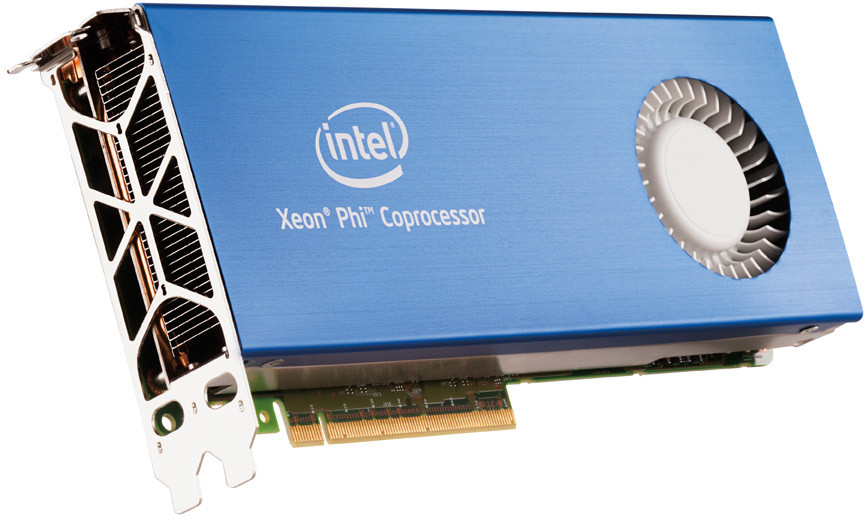
\includegraphics[width=0.99\textwidth]{figures/xeon-phi.jpg} \\[1.5em]
 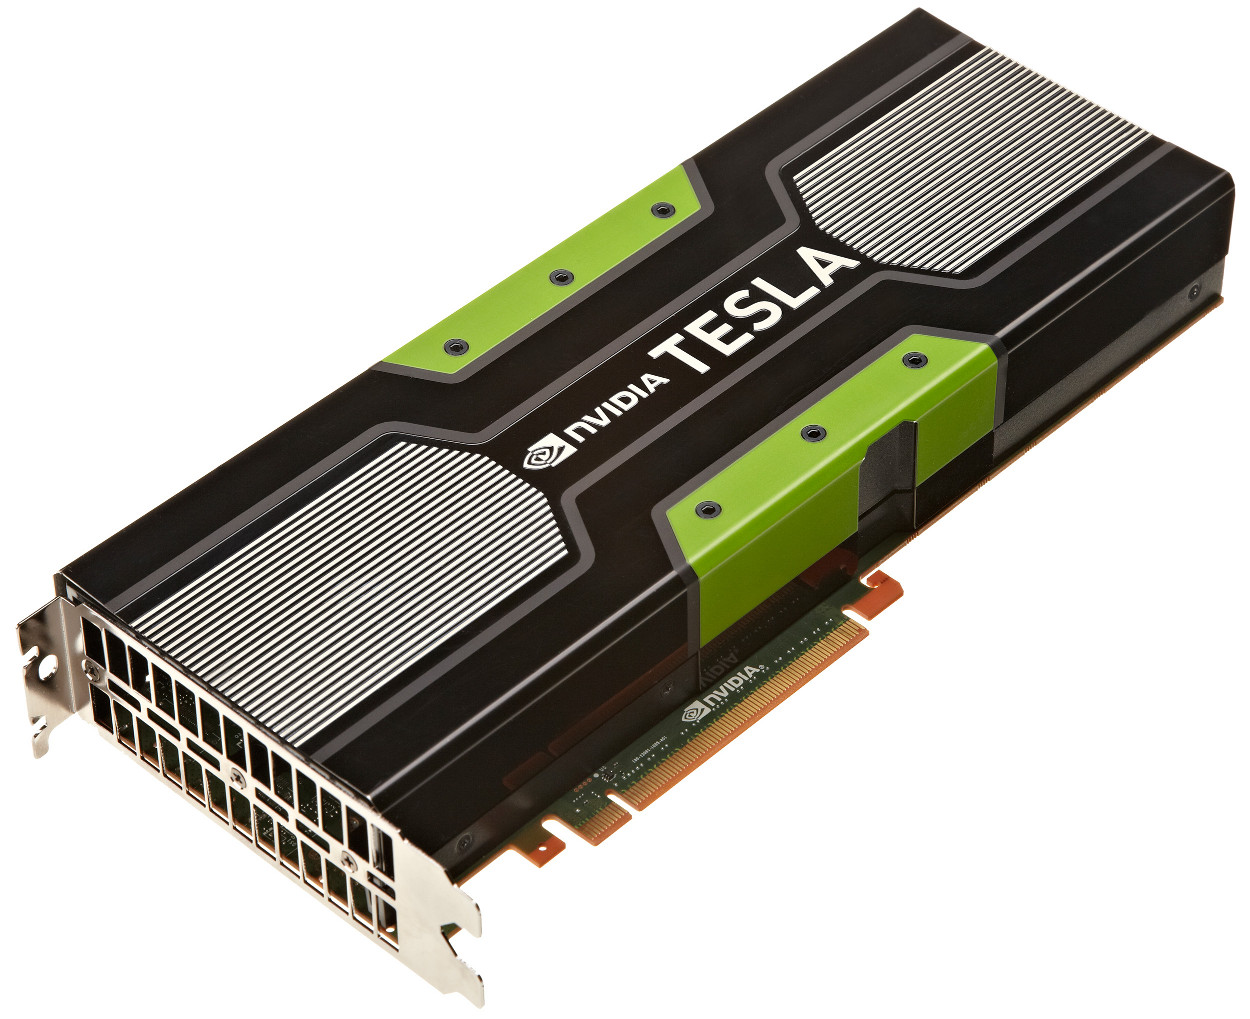
\includegraphics[width=0.99\textwidth]{figures/TeslaK20.jpg} \\[1.5em]
 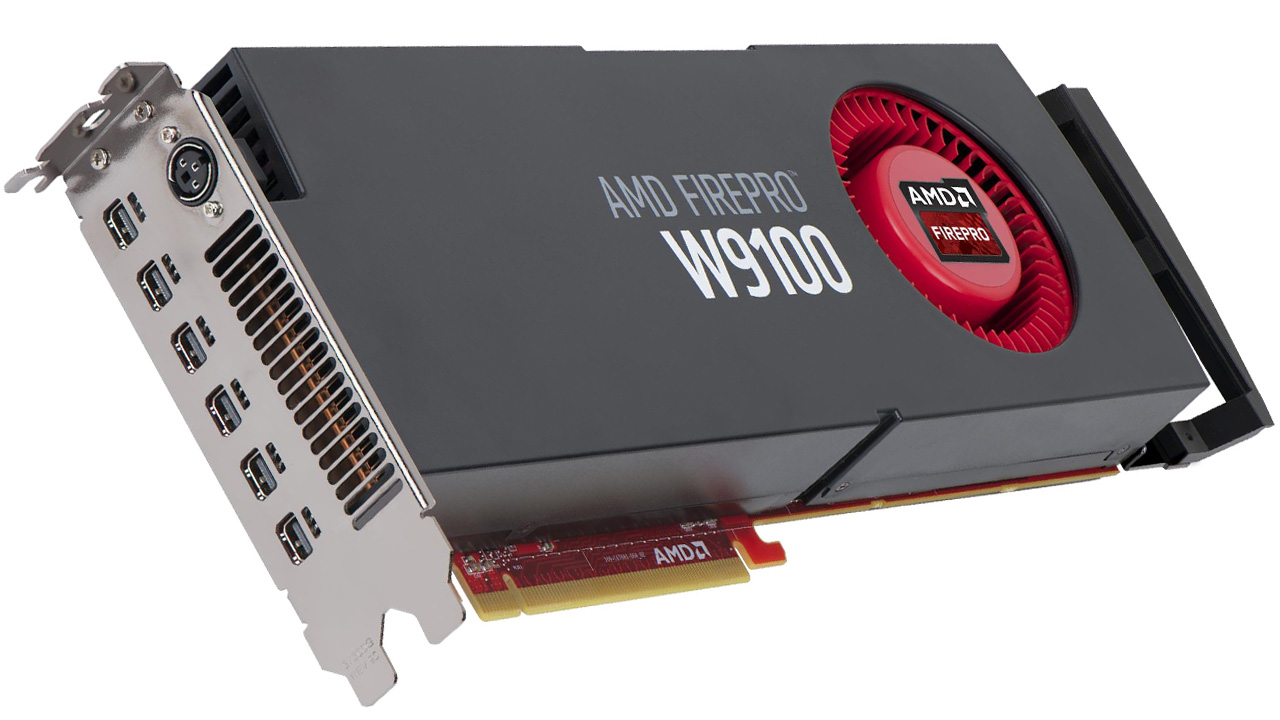
\includegraphics[width=0.99\textwidth]{figures/w9100.jpg} \\[1.5em]
 \end{minipage}


\end{frame}


% Configure PETSc
\begin{frame}[fragile]
\frametitle{Configuration}
  \begin{block}{CUDA (CUSP)}
    \begin{itemize}
     \item CUDA-enabled configuration (minimum)
     \begin{lstlisting}
 ./configure [..] --with-cuda=1
   --with-cusp=1 --with-cusp-dir=/path/to/cusp
     \end{lstlisting}
     \item Customization:
     \begin{lstlisting}
   --with-cudac=/path/to/cuda/bin/nvcc
   --with-cuda-arch=sm_60
     \end{lstlisting}
    \end{itemize}
  \end{block}
  
  \begin{block}{OpenCL (ViennaCL)}
    \begin{itemize}
     \item OpenCL-enabled configuration
     \begin{lstlisting}
 ./configure [..] --download-viennacl
    --with-opencl-include=/path/to/OpenCL/include
    --with-opencl-lib=/path/to/libOpenCL.so
     \end{lstlisting}
    \end{itemize}
  \end{block}
\end{frame}


% How does it work?
\begin{frame}[fragile]
\frametitle{How Does It Work?}
  \begin{block}{Host and Device Data}
  \begin{lstlisting}
struct _p_Vec {
  ...
  void          *data;            // host buffer
  PetscCUSPFlag valid_GPU_array;  // flag
  void          *spptr;           // device buffer
};
  \end{lstlisting}
  \end{block}

  \begin{block}{Possible Flag States}
  \begin{lstlisting}
  typedef enum {PETSC_CUSP_UNALLOCATED,
                PETSC_CUSP_GPU,
                PETSC_CUSP_CPU,
                PETSC_CUSP_BOTH} PetscCUSPFlag;
  \end{lstlisting}
  \end{block}

\end{frame}

\begin{frame}[fragile]
\frametitle{How Does It Work?}

  \begin{block}{Fallback-Operations on Host}
   \begin{itemize}
    \item Data becomes valid on host (\lstinline|PETSC_CUSP_CPU|)
      \begin{lstlisting}
PetscErrorCode VecSetRandom_SeqCUSP_Private(..) {
  VecGetArray(...);
  // some operation on host memory
  VecRestoreArray(...);
}
      \end{lstlisting}
   \end{itemize}
  \end{block}

  %\pause 
  
  \begin{block}{Accelerated Operations on Device}
   \begin{itemize}
    \item Data becomes valid on device (\lstinline|PETSC_CUSP_GPU|)
      \begin{lstlisting}
PetscErrorCode VecAYPX_SeqCUSP(..) {
  VecCUSPGetArrayReadWrite(...);
  // some operation on raw handles on device
  VecCUSPRestoreArrayReadWrite(...);
}
      \end{lstlisting}
   \end{itemize}
  \end{block}

\end{frame}


% Example with ILU
\begin{frame}[fragile]
\frametitle{Example}
  \begin{block}{KSP ex12 on Host}
  \begin{itemize}
   \item
    \begin{lstlisting}
$> ./ex12
    -pc_type ilu -m 200 -n 200 -log_summary
    \end{lstlisting}
    \begin{lstlisting}
KSPGMRESOrthog       228 1.0 6.2901e-01
KSPSolve               1 1.0 2.7332e+00
    \end{lstlisting}

  \end{itemize}
  \end{block}

  %\pause
  
  \begin{block}{KSP ex12 on Device}
  \begin{itemize}
   \item
    \begin{lstlisting}
$> ./ex12 -vec_type cusp -mat_type aijcusp
    -pc_type ilu -m 200 -n 200 -log_summary
    \end{lstlisting}
    \begin{lstlisting}
[0]PETSC ERROR: MatSolverPackage petsc does not support matrix type seqaijcusp
    \end{lstlisting}

  \end{itemize}
  \end{block}
  \vspace*{0.4cm}

\end{frame}


% Example without preconditioner
\begin{frame}[fragile]
\frametitle{Example}
  \begin{block}{KSP ex12 on Host}
  \begin{itemize}
   \item
    \begin{lstlisting}
$> ./ex12 
    -pc_type none -m 200 -n 200 -log_summary
    \end{lstlisting}
    \begin{lstlisting}
KSPGMRESOrthog      1630 1.0 4.5866e+00
KSPSolve               1 1.0 1.6361e+01
    \end{lstlisting}

  \end{itemize}
  \end{block}

  %\pause
  
  \begin{block}{KSP ex12 on Device}
  \begin{itemize}
   \item
    \begin{lstlisting}
$> ./ex12 -vec_type cusp -mat_type aijcusp
    -pc_type none -m 200 -n 200 -log_summary
    \end{lstlisting}
    \begin{lstlisting}
MatCUSPCopyTo          1 1.0 5.6108e-02
KSPGMRESOrthog      1630 1.0 5.5989e-01
KSPSolve               1 1.0 1.0202e+00
    \end{lstlisting}

  \end{itemize}
  \end{block}

\end{frame}


% Pitfalls
\begin{frame}[fragile]
\frametitle{Pitfalls}
  \begin{block}{Pitfall: Repeated Host-Device Copies}
  \begin{itemize}
   \item PCI-Express transfers kill performance
   \item Complete algorithm needs to run on device
   \item Problematic for explicit time-stepping, etc.
  \end{itemize}
  \end{block}

  %\pause
  
  \begin{block}{Pitfall: Wrong Data Sizes}
  \begin{itemize}
   \item Data too small: Kernel launch latencies dominate
   \item Data too big: Out of memory
  \end{itemize}
  \end{block}

  %\pause
  
  \begin{block}{Pitfall: Function Pointers}
  \begin{itemize}
   \item Pass CUDA function ``pointers'' through library boundaries?
   \item OpenCL: Pass kernel sources, user-data hard to pass
   \item Composability?
  \end{itemize}
  \end{block}

\end{frame}



% Pitfalls
\begin{frame}[fragile]
\frametitle{Pitfalls}
  \begin{block}{Pitfall: GPUs are too fast for PCI-Express}
  \begin{itemize}
   \item Latest GPU peaks: 720 GB/sec from GPU-RAM, 16 GB/sec for PCI-Express
   \item 40x imbalance (!)
  \end{itemize}
  \end{block}

  %\pause
  \begin{center} \vspace*{-1.0cm}
    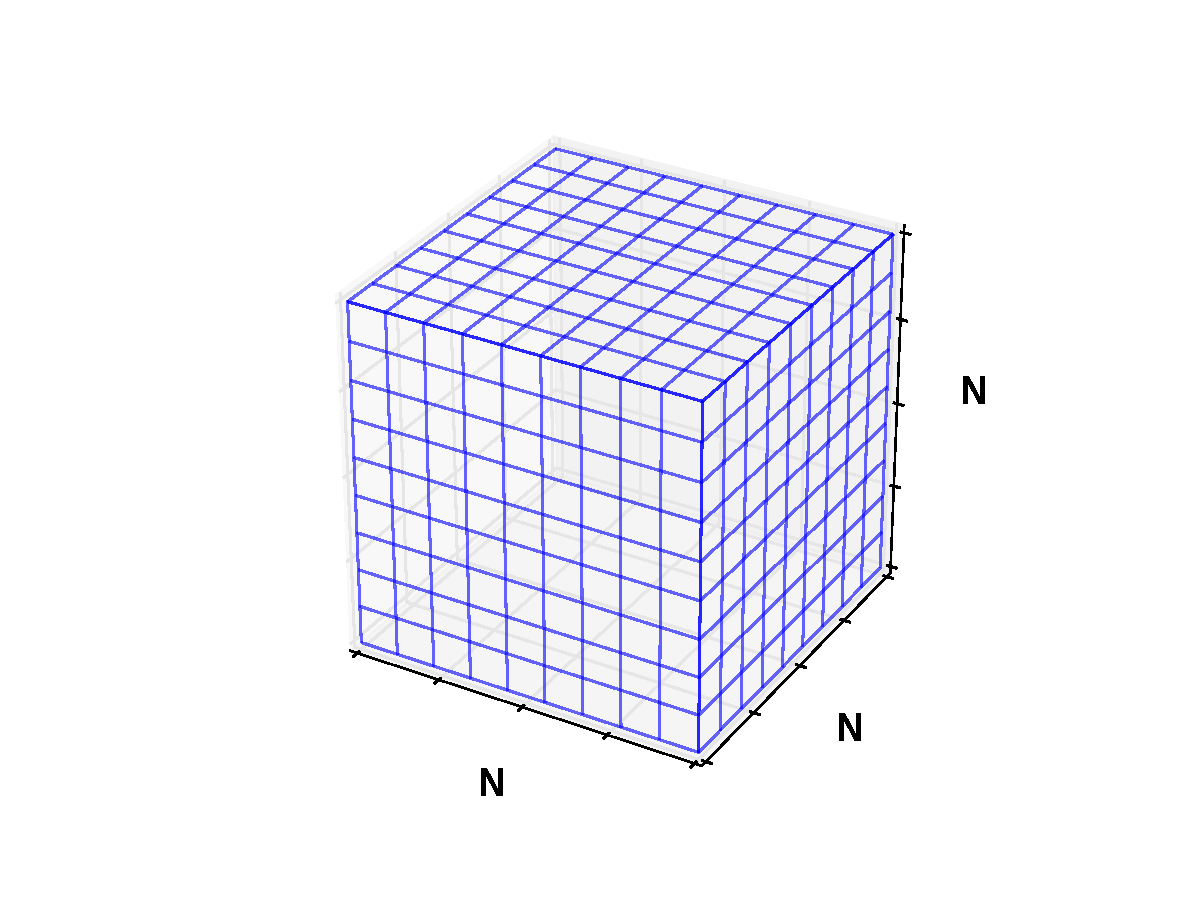
\includegraphics[width=0.5\textwidth]{figures/cube-discretization}
  \end{center}

  %\pause
  \vspace*{-0.5cm}
   \begin{block}{Compute vs. Communication}
  \begin{itemize}
   \item Take $N=512$, so each field consumes 1 GB of GPU RAM
   \item Boundary communication: $2 \times 6 \times N^2$: 31 MB
   %\pause
   \item Time to load field: 1.4 ms
   %\pause
   \item Time to load ghost data: \textbf{1.9 ms (!!)}
  \end{itemize}
  \end{block}

\end{frame}


\begin{frame}{PETSc and GPUs}
   \begin{center} \Large \textbf{Many PETSc Operations \\[1em] do NOT benefit from modern high-end GPUs \\[1em] in a substantial way!}\\ \scriptsize (Exception: OpenPower systems) \end{center}
\end{frame}


% Overview of what is available
\begin{frame}[fragile]
\frametitle{Current GPU-Functionality in PETSc}
  
  \begin{block}{Current GPU-Functionality in PETSc}
  \begin{center}
  \renewcommand{\arraystretch}{1.2}
  \begin{tabular}{|l|c|c|}
   \hline
                     & \textbf{CUSP/CUDA}  & \textbf{ViennaCL} \\
   \hline
   Programming Model & CUDA                & CUDA/OpenCL/OpenMP \\
   \hline
   Operations        & Vector, MatMult     & Vector, MatMult \\
   \hline
   Matrix Formats    & CSR, ELL, HYB       & CSR \\
   \hline
   Preconditioners   & SA-AMG, BiCGStab    & SA/Agg-AMG, Par-ILU0 \\
   \hline
   MPI-related       & Scatter             & - \\
   \hline
  \end{tabular}
  \end{center}
  \end{block}

  \begin{block}{Additional Functionality}
   \begin{itemize}
    \item MatMult via cuSPARSE
    \item OpenCL residual evaluation for PetscFE
   \end{itemize}
  \end{block}


\end{frame}


